\documentclass[../main.tex]{subfiles}

\begin{document}

\chapter{System Design}\label{ch:system-design}

This chapter describes the design of the proposed monitoring system. 
It first derives the requirements that follow from the research questions and the preceding chapter, 
and then presents the system along the path that data takes through it. 
First, the data aggregation inside the IdP. 
Then, the transport of the collected data across a trust boundary. 
Finally, storage, correlation and rule-based detection.

The emphasis lies on the collection layer. 
The remaining layers follow established practice, whereas the question of which data can be obtained 
from within an identity provider, and by which mechanisms, is specific to this work. 
Design decisions are stated together with the alternatives that were considered and rejected.

\section{Requirements for the System}\label{sec:requirements}

The requirements for the monitoring system were derived from the research and analysis of the related work.
Section~\ref{sec:why-not-siem} showed that AppSensor's detection model provides no mechanism for 
comparing an observed event against a configuration declared by a third party. 
Since an IdP authenticates on behalf of other entities, such a comparison requires at least two 
independent sources.
One source describing the intended configuration and another describing what actually occurred.

The classification in Section~\ref{sec:why-inside} placed this work at the \textit{Monitor and Detect} 
level, with \textit{Plan and Prevent} deliberately excluded. 
The system must therefore report detected security-relevant events without automatically intervening.

As mentioned in Section~\ref{sec:why-inside}, Hall et al. identify the integration of detection 
points into the application as a central difficulty~\cite{BlackWatch}. 
The system is therefore implemented as a plugin that uses an extension point provided by Shibboleth, 
allowing the monitoring functionality to be added without modifying the underlying IdP implementation. 

Section~\ref{sec:why-not-siem} also showed that log sources stored on the same system share the 
same attack surface. 
Records generated by the interceptor are therefore transmitted to a separate system rather than 
stored locally. 
This requires the transport to be authenticated and sensitive data to be pseudonymised at the source.

The rules presented in Section~\ref{sec:rules}, derived from the FIM survey by Simpson and Groß, the 
OASIS SAML Security and Privacy Considerations, and the STRIDE threat classification scheme, provide 
the actual detection logic for identifying unusual authentication behaviour and security-relevant 
conditions within the federated identity environment. 

These considerations result in five requirements:
\begin{enumerate}
    \item Two independent sources: the declared configuration and the observed event.
    \item Detection and reporting without automated intervention.
    \item Realisation as a plugin, without modification of the identity provider.
    \item Storage outside the monitored system, with authenticated transport and pseudonymisation at the source.
    \item Detection rules derived from documented attack classes and normative requirements.
\end{enumerate}

\section{Overview}\label{sec:overview}

The proposed system comprises four layers. 
The data collection layer gathers security-relevant information from within the Shibboleth IdP, 
drawing on three sources: the audit log written by the IdP, its static configuration and metadata files, 
and a custom interceptor executing inside the IdP itself. 
Because the monitoring backend resides outside the trust boundary of the IdP, sensitive attributes such 
as usernames and IP addresses are pseudonymised before transmission. 
The transport layer then transfers the collected records to the backend application over an authenticated channel. 
Within the backend, incoming records are persisted and periodically correlated, so that observations 
originating from different sources but describing the same authentication event can be linked. 
The detection layer evaluates the resulting data against the rule catalogue in order to identify 
configuration weaknesses and anomalies in the authentication process. 
Finally, the presentation layer makes the detected findings accessible to the operator through a frontend 
web application.
Figure~\ref{fig:deployment} illustrates the UML deployment diagram of the proposed system. 

\begin{figure}[ht]
    \centering
    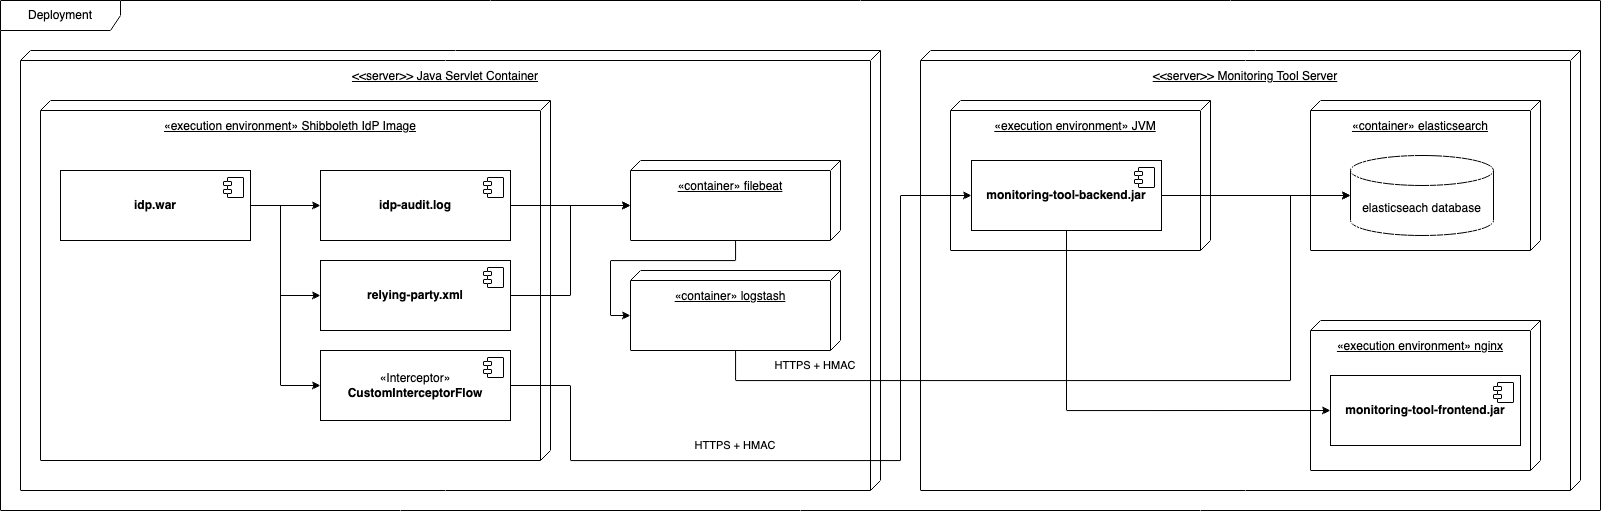
\includegraphics[width=\textwidth]{../img/deployment}
    \caption{UML-Deployment-Diagram of the Shibboleth Identity Provider Monitoring Tool}
    \label{fig:deployment}
\end{figure}

\section{Data Aggregation Layer}\label{sec:data-aggregation}

The design of the collection layer begins with a broader question than the choice of individual data sources. 
Through which kinds of channel does an application disclose information about itself at all?
Applied to the Shibboleth IdP, five such channels can be identified. 
The application writes log files, it reads static configuration and metadata, it maintains runtime state that 
is accessible through defined extension points, it exposes status endpoints, and it publishes metrics via Java 
Management Extensions. 

Not all of these are suitable for the purpose of this work. 
The system described here associates every finding with an individual authentication event, since a security 
relevant condition is only meaningful in the context of the transaction in which it occurred. 
A channel that cannot be related to a single login can therefore not contribute to correlation or to the 
generation of an alert. 

Two of the five channels fail this criterion. 
Status endpoints report the state of the deployment as a whole, such as its version, uptime, configured metadata 
providers or the status of the underlying services. 
They therefore address availability rather than the security of individual transactions. 
JMX metrics are aggregates by construction. 
A counter reports that a number of logins occurred, not which login was affected. 
An alert derived from either source could not be attributed to a transaction. 

The remaining three channels form the collection layer of this work. 
These are the audit log, the configuration files, and the runtime state accessible through an interceptor. 
They are described in the following sections. 

\subsection{The Audit Logs}\label{subsec:audit-log}

All logging within the Shibboleth IdP is performed through the abstract logging API SLF4J, 
with Logback as the default implementation. 
By default, three classes of log files are produced. 
The diagnostic logs, \textit{idp-process.log} and \textit{idp-warn.log}, contain messages generated during 
the normal operation of the software. 
The general audit log, \textit{idp-audit.log}, records the results of authentication transactions for each SP. 
Finally, the consent audit log, \textit{idp-consent-audit.log}, contains audit records of user decisions 
regarding data privacy and terms of use~\cite{LoggingConfiguration}.

The amount of information recorded in the diagnostic logs depends on the configured logging 
level, which determines the severity of messages that are written. 
The \textit{idp-warn.log} file is a filtered view of \textit{idp-process.log} and contains 
only messages logged at the \texttt{WARN} level or higher.

In contrast to the diagnostic logs, the audit log is intended to be machine readable. 
It records one entry per completed transaction, written once the IdP has finished processing 
the request. 
This has two consequences for the information it can provide. 
On the one hand, the entry reflects the final outcome of a transaction, including properties 
that are only determined at the end of processing, such as the encryption applied to the 
outgoing assertion. 
On the other hand, events that never result in a completed transaction produce no entry. 
Failed password validations in particular are not recorded in the audit log, since the 
authentication flow terminates before a transaction is concluded.

As mentioned in Section~\ref{subsec:audit-logging}, the fields that are written to the audit 
log are not fixed. 
The audit format is configured per profile in \textit{conf/audit.xml}, where each field is 
represented by a formatting token, and the set of available tokens can be extended within the 
IdP~\cite{AuditLoggingConfiguration}. 
Which information a given deployment records is therefore determined by its administrator and 
may differ between installations. 

This property has direct implications for the monitoring system developed in this work. 
The system cannot assume the presence of a fixed set of audit fields, since the information 
required by a particular detection rule may simply not be recorded. 
The detection logic must therefore take the configured audit format into account and determine 
whether the information a given rule depends on is available at all. 
The same constraint applies to the correlation between audit entries and interceptor records. 
Rather than relying on a fixed set of fields, the correlation must adapt to the information 
that a given deployment provides, which requires a strategy capable of selecting an appropriate 
matching approach depending on the fields available for a given audit event.

\subsection{Metadata and Relying Party File}\label{subsec:static-configuration}

In a Shibboleth IdP, SAML metadata describes the entities that participate in a federation 
and provides the information required for establishing communication between them. 
Metadata is represented in XML and contains information about the roles, endpoints, supported 
protocols, and cryptographic keys of the participating entities~\cite{Metadata}.

A SAML entity can support one or more roles, which are represented by role descriptors within 
the metadata. 
For SPs, the relevant role is represented by the \texttt{md:SPSSODescriptor} element. 
This descriptor contains information required by the IdP to communicate with the SP, including 
the supported SAML protocol families specified by the \texttt{protocolSupportEnumeration} 
attribute, cryptographic keys, supported name identifier formats, and the endpoints provided 
by the SP~\cite{MetadataForSP}.
A central component of an SP's metadata is the \texttt{md:AssertionConsumerService} element. 
It specifies an endpoint to which the IdP can send SAML responses and assertions on behalf 
of the SP. 
By explicitly enumerating these endpoints in the metadata, the IdP can determine the locations 
to which SAML messages may be sent~\cite{MetadataForSP}.

The Shibboleth IdP consumes metadata through configured metadata providers. 
These providers define the sources from which SAML metadata is obtained and are configured using 
\texttt{<MetadataProvider>} elements in \textit{conf/metadata-providers.xml}~\cite{MetadataConfiguration}. 
The metadata therefore forms an essential part of the IdP configuration, as it determines which 
federation entities are known to the IdP and which endpoints, protocols, and cryptographic 
information are associated with them. 

Alongside the runtime information recorded in the audit log, the IdP holds a second class of 
information that describes not what happened, but what is supposed to happen. 
This information is contained in the configuration files of the deployment, most notably in 
\textit{relying-party.xml}.

This file specifies which functional features the IdP supports and allows these settings to be 
customised based on the identity of a relying party. 
It determines which profiles are enabled for a given partner and allows security configurations 
to be attached at various levels. 
These include whether assertions and other content are encrypted, at which layer signing is 
performed, and which cryptographic algorithms are used~\cite{RelyingPartyConfiguration}.

Of particular relevance to this work is that these settings are not global. 
A deployment defines default behaviour that applies to all partners, and may then override this 
behaviour for individual relying parties or groups of them. 
A single IdP therefore enforces a set of independent, per partner policies rather than one uniform 
policy, and the security properties of a given transaction depend on which policy applies to the 
SP involved. 

Two settings are relevant in the context of this work. 
The first concerns encryption. 
A deployment may disable the encryption of assertions for a particular partner, for instance where 
a SP does not support it, which means that assertions for that partner are transmitted 
in plain text. 
The second concerns authentication. 
A deployment may specify which authentication flows are permitted for a partner, and thereby 
require multi factor authentication for some SP while accepting password based authentication 
for others.

Both settings describe a target state. 
Whether a given login actually satisfied it is recorded in the audit log, not in the configuration. 
Neither source is sufficient on its own. 
A comparison between them is only possible if both are available to the monitoring system, which 
is the reason why the configuration is treated as an independent data source in this work.

Finally, \textit{relying-party.xml} is also the file in which interceptor flows are enabled for a 
profile. 
The extension point used by the collection mechanism described in 
Section~\ref{subsec:interceptor} is therefore configured in the same place as the security settings 
it observes.

\subsection{Interceptor}\label{subsec:interceptor}

As mentioned Section~\ref{subsec:profile-flows} Shibboleth provides three interception points 
within its profile processing: inbound message processing, post-authentication processing, and 
outbound message processing. 
Interceptors are implemented as Spring Web Flow subflows that are executed at these predefined 
points without requiring modifications to the underlying profile 
flow~\cite{ProfileHandling, ProfileInterceptConfiguration}.

Inbound interceptors are executed during the processing of an incoming request. 
At this point, the inbound \texttt{MessageContext} tree is generally populated and, where 
applicable, contains a \texttt{RelyingPartyContext} as well as contexts required for operations 
such as transport or message authentication~\cite{ProfileHandling}.

Consequently, an inbound interceptor can observe information associated with the received message 
and the context in which it is being processed. 
This makes the interception point particularly suitable for security checks on the incoming request. 
Shibboleth itself uses inbound interceptors for various security policy checks. 
An interceptor may also modify the context tree, although such modifications directly influence 
subsequent profile processing~\cite{ProfileHandling}.

For the monitoring system developed in this work, the inbound interception point is therefore relevant 
for observing properties of the incoming SAML message and its processing context before the main 
profile execution continues.

The post-authentication interception point is executed after authentication and attribute lookup have 
taken place, but before the profile constructs the outgoing message. 
Unlike the inbound and outbound hooks, this interception point is only available for a subset of 
profiles, particularly profiles that perform user authentication~\cite{ProfileHandling}.

The interceptor therefore has access to a later state of the processing context. 
In particular, information related to the authenticated identity and resolved attributes is available 
at this stage. 
The interceptor can also modify the context before the outgoing response is constructed, including 
changes to the authenticated identity or attributes~\cite{ProfileHandling}. 

This makes the post-authentication interception point particularly suitable for the monitoring system 
developed in this work, as it provides access to authentication-related information that is not yet 
available at the inbound stage while still allowing the resulting SAML response to be observed 
indirectly through the processing context.

Outbound interceptors run shortly before the final stage of profile processing that produces the 
response to the client. 
Their input therefore represents the state produced by the preceding profile execution and typically 
contains a populated outbound \texttt{MessageContext}. 
The message may not yet be in its final form, since operations such as signing can still occur 
afterwards~\cite{ProfileHandling}.

The outbound interception point consequently provides access to the information that is about to 
be returned to the relying party. 
Interceptors can inspect or modify the outbound context and may also terminate processing~\cite{ProfileHandling}.
For the monitoring system, this interception point is useful for observing the result of the 
authentication workflow and properties of the response that is about to be issued by the IdP.

The monitoring system uses the post-authentication interception point. 
This choice determines what the collection mechanism can observe. 
An inbound interceptor would see the incoming message but not the outcome of authentication, 
since that has not yet taken place. 
An outbound interceptor would see the response about to be issued, but the request that caused 
it is no longer the object of processing at that stage. 
The post-authentication point is the only one at which both the incoming message and the 
authentication result are available in the same context.

What remains outside its view is the outgoing response, including the assertion identifier, 
the encryption actually applied and the final status of the transaction. 
These properties are recorded in the audit log, which is written after the transaction 
has completed. 
The complementarity of the two sources described in Section~\ref{subsec:audit-log} therefore 
follows from their position in the processing sequence rather than from a deliberate 
division of responsibilities.

\section{Transport Layer and Trust Boundary}\label{sec:trust}

After the data has been aggregated on the Shibboleth IdP side, it is transferred to the 
monitoring tool for further processing and storage. 
As stated in Section~\ref{sec:overview}, this tool is deliberately deployed outside the 
trust boundary of the IdP. 
The separation avoids placing the monitoring system under the same security assumptions 
and access controls as the system it monitors. 

If the monitoring functionality were deployed entirely within the IdP, an attacker who compromises 
the IdP could potentially compromise or manipulate the monitoring functionality at the same time. 
An attacker would then be in a position to influence the recording of their own activity, 
since collection, storage and analysis would all fall under the same control. 

By transferring the collected information to a separate monitoring component, the observation 
and analysis functions are separated from the monitored application. 
This creates an additional security boundary and reduces the dependency of the monitoring system 
on the integrity of the IdP itself.
The external component therefore does not exist solely for scalability or architectural 
convenience. 
What the separation protects is the data that has already been transmitted. 
An attacker who gains control of the IdP can influence which records are produced from that point 
onward, but not those that have already left the system. 
The independence is thus temporal rather than absolute. 

This design decision has consequences. 
The collected data leaves the security domain in which the original authentication 
data is processed and becomes accessible to a separate component with a different trust 
relationship. 
Therefore, transmitting original sensitive user information, such as usernames and client IP addresses, 
would expose more personal information than is necessary for the intended processing purpose. 
A comparable concern is described by CWE-532 for log files, where the inclusion of sensitive user data 
provides attackers with an additional and less protected path to obtaining that information~\cite{CWE532}. 
The same reasoning applies to data transferred to a component outside the original security domain.

To reduce this exposure, sensitive identifiers are pseudonymised before they leave the IdP trust boundary. 
The monitoring functionality does not require the original identity of a user to perform its security analysis. 
It primarily requires the ability to distinguish and correlate events belonging to the same subject. 
The monitoring system can therefore preserve the ability to correlate multiple events belonging to the same 
subject without transmitting the original identifier. 
Pseudonymisation reduces the risk associated with unauthorised access to the monitoring system, while still 
allowing the required security analysis to be performed. 

To enable this correlation across the different data sources, all components that generate monitoring data 
must apply the same pseudonymisation algorithm and the same secret salt. 
Otherwise, identical identifiers would result in different pseudonyms and events originating from different 
sources could no longer be reliably correlated. 
The secret salt is therefore treated as a shared cryptographic parameter between the data collection components 
and must be protected accordingly. 

The deployment of the monitoring tool outside the IdP trust boundary introduces an additional security concern. 
The endpoints of the monitoring tool accept data from collection components that reside outside its own 
trust boundary. 
Consequently, the monitoring tool cannot assume that every received message originates from an authorised data 
collection component.

Without message authentication, an attacker could submit forged or manipulated records to the exposed endpoints. 
Injected events would not only produce false findings but could also interfere with the correlation of genuine 
ones, since a fabricated record may be matched against a real audit entry.

The transmitted data must therefore be authenticated before the monitoring tool accepts it. 
In this work, this is achieved using a \gls{hmac}. 
The collection components and the monitoring tool share a secret key that is used to generate and verify a 
message authentication code for each transmitted message.

The final design decision concerning the transport layer is whether the collection component should wait for 
the monitoring tool to confirm receiving the data.
The interceptor executes within the authentication flow of the IdP. 
Any time spent transmitting a record is therefore time added to the login of the user who triggered it. 
Waiting for a response would make the duration of every authentication dependent on the availability and 
response time of a component outside the IdP, and a monitoring tool that is slow or temporarily unreachable 
would delay the service it observes.

The records are consequently transmitted asynchronously. 
The interceptor dispatches the record and continues processing without awaiting a response.
This has a cost. 
If a transmission fails, the collection component does not learn of it, and the record is lost without 
any indication at the point where it originated. 
The design therefore prioritises non interference with the monitored service over a guarantee of delivery. 
For a monitoring system that observes a central authentication service, this trade off appears justified. 
A monitoring component that degrades the availability of the service it observes would undermine its own purpose. 
Hall et al. arrive at the same decision for the same reason, transmitting detection events separately rather 
than in response to the triggering request so that analysis does not delay the monitored 
application~\cite{BlackWatch}. 

\section{Correlation and Detection Layer}\label{sec:processing}

This section explains how the monitoring tool processes the collected data. 
Records originating from different sources are first linked to the authentication event they describe, then 
evaluated against the detection rules, and finally classified according to the impact of the condition they report.

\subsection{Correlation}\label{subsec:correlation}

When the collected data arrives at the monitoring tool, it must first be stored for subsequent 
processing. 
The different data sources transmit their information through separate endpoints and at 
different times, which means that information belonging to the same authentication event does 
not necessarily arrive together. 
The corresponding records can therefore not always be correlated upon arrival. 
Instead, they are stored until the required information from the other source becomes available.

This introduces the first challenge for the correlation process. 
Data collected by the custom interceptor within the Shibboleth IdP is transmitted immediately 
after the collection process has completed, so the corresponding report reaches the monitoring 
tool shortly after the authentication event has been processed. 
The audit entry follows a different path. 
Audit logs are collected by log shippers that operate periodically, and the corresponding entry 
therefore reaches the monitoring tool later than the interceptor report. 
This temporal offset is the reason why the two records cannot be matched by a simple database 
join at the time of arrival.

A further consequence follows from this. 
A report may arrive at a point when its counterpart does not yet exist, which means that an 
unsuccessful correlation attempt does not necessarily indicate that no counterpart will ever 
arrive. 
The correlation process must therefore retry over a defined period and, once that period has 
elapsed, treat the record as permanently uncorrelated. 
Without this distinction, a record still awaiting its counterpart would be indistinguishable 
from one that will never receive it, and the proportion of successfully correlated records 
could not be determined.

The second challenge arises from the dynamic nature of the audit log discussed in 
Section~\ref{subsec:audit-log}. 
Since the audit format is determined by the configuration of the deployment, the information 
available in an audit record is not fixed, and the correlation must adapt to the fields that 
are actually present.

This creates an asymmetric correlation problem. 
The data collected by the custom interceptor is static by design and always contains the same 
set of fields. 
The audit data, in contrast, is dynamic and may lack information required by a particular 
correlation strategy. 
The static interceptor report, which arrives first, therefore has to be matched against a 
dynamic audit record that arrives later.

Depending on the fields available in the audit record, different correlation strategies are 
applicable, and these differ in how reliably they identify the corresponding record. 
A strategy based on a unique identifier that both sources share establishes the relationship 
unambiguously, whereas a strategy based on attributes that several transactions may have in 
common can only approximate it. 
The correlation process consequently applies the available strategies in a defined priority 
order, using the strongest applicable strategy first and weaker ones only where the required 
fields are absent. 
The strategy used for a given record is recorded alongside the result, since it determines how 
reliable the resulting correlation is. 
The precision achieved by each strategy is examined in Chapter~\ref{ch:evaluation}.

\subsection{Detection}\label{subsec:detection}

Once the data has been collected and stored, it is evaluated against a catalogue of detection 
rules, where possible. 
A rule receives a single object as input and either returns a finding or nothing. 
The conditions are stated explicitly rather than learned from data, which means that every 
finding can be traced back to the condition that produced it and, through the derivation in 
Section~\ref{sec:rules}, to the documented weakness or requirement it is based on. 

The rules do not all operate on the same kind of input. 
Four input types occur in this system: login events derived from the audit log, the configuration 
of a service provider, its metadata, and the reports produced by the interceptor. 
These differ not only in structure but also in the rhythm at which they appear. 
Login events occur continuously during operation, whereas a configuration or a metadata document 
changes rarely and may remain unchanged for long periods of time.

Evaluating all rules against all data whenever any of it changes would therefore be inefficient 
and, in the case of configuration data, largely redundant. 
The detection logic is consequently divided into four engines, each responsible for one input 
type. 
An engine evaluates the rules that apply to its input and can be scheduled according to the 
frequency at which that input actually changes.

A further consideration follows from the dynamic audit format described in 
Section~\ref{subsec:audit-log}. 
A rule may depend on a field that a given deployment does not record, in which case the rule 
cannot reach a valid conclusion. 
Evaluating it regardless would produce a result that appears definite but rests on absent 
information, and a rule that cannot observe a condition must not report its absence as a finding. 
Each rule therefore declares which fields it requires, and the engine verifies their availability 
before evaluating the rule. 
Where the required information is not recorded, the rule withdraws rather than returning a 
result. 
Which rules are active in a given deployment is thus determined by what that deployment logs. 

Which conditions the rules examine is a separate question from how they are evaluated. 
The catalogue of thirteen rules was derived from the three frameworks introduced in 
Section~\ref{sec:rules}, namely the survey by Simpson and Groß, the OASIS security 
considerations and the STRIDE classification. 
Table~\ref{tab:rules} shows the resulting assignment for each rule.

\begin{table}[h]
\centering
\caption{Assignment of the 13 Detection Rules to Documented Vulnerabilities and Attack Classes}\label{tab:rules}
\small
\begin{tabular}{p{3.3cm}p{2.7cm}p{2.4cm}p{1.1cm}l}
\toprule
Rule & Vulnerability & Attack Class & STRIDE & Source \\
\midrule
WEAK\_ENCRYPTION                                     & Unencrypted Communications & Message Modification     & I, T    & \cite{FIMSurvey,BSITR02102,SAMLSecurityConsideration} \\
UNENCRYPTED\_\linebreak ASSERTION                    & Unencrypted Communications & Message Modification     & I, T    & \cite{FIMSurvey,ShibbolethGIAC} \\
WEAK\_\linebreak CONFIGURATION                       & Unencrypted Communications & Message Modification     & I, T    & \cite{FIMSurvey} \\
MISSING\_MFA                                         & Weak User Credentials      & Enables Brute Force      & S, E    & \cite{FIMSurvey} \\
MFA\_BYPASS                                          & Weak User Credentials      & Enables Brute Force      & S, E    & \cite{FIMSurvey} \\
BRUTE\_FORCE                                         & Weak User Credentials      & Brute Force              & S, E    & \cite{FIMSurvey} \\
FAILED\_LOGIN                                        & Weak User Credentials      & Indicator, not an attack & S       & \cite{OWASPA09} \\
ASSERTION\_REPLAY                                    & Lack of Binding            & Replay Attack            & S, E    & \cite{FIMSurvey,SAMLSecurityConsideration} \\
REQUEST\_REPLAY                                      & Lack of Binding            & Replay Attack            & S, E    & \cite{FIMSurvey,SAMLSecurityConsideration} \\
SIGNATURE\_\linebreak WRAPPING\_\linebreak SUSPECTED & Message Formatting         & Message Modification     & S, T, E & \cite{BreakingSAML,ShibbolethGIAC} \\
CERTIFICATE\_\linebreak EXPIRED                      & None                       & None                     & S       & \cite{SAMLSecurityConsideration} \\
SUSPICIOUS\_\linebreak USER\_AGENT                   & None                       & None                     & ---     & --- \\
BEHAVIOUR\_\linebreak ANOMALY                        & Multiple                   & Detection method         & S       & --- \\
\bottomrule
\end{tabular}
\end{table}

Two observations follow from this assignment. 
Lack of binding appears in three of the six SAML related entries and is therefore the most frequently 
documented weakness of the protocol in the survey. 
Both replay rules address it directly. 
Furthermore, several rules form pairs in which the same weakness is captured twice, once as a 
configuration state and once as an event that has occurred. 
MISSING\_MFA examines whether a service provider requires multi factor authentication at all, whereas 
MFA\_BYPASS examines whether an actual login circumvented that requirement. 
This distinction is a direct consequence of the three source architecture described in 
Section~\ref{sec:data-aggregation}: the configuration states what is intended, and the audit log 
records what took place.

Two rules cannot be assigned to any of the three frameworks. 
SUSPICIOUS\_USER\_AGENT identifies an indicator for which no documented relation to a specific attack 
class could be established. 
BEHAVIOUR\_ANOMALY is a detection method rather than an attack class, since it may reveal several 
different attacks indirectly without corresponding to any one of them. 
Both rules are retained in the catalogue, and the absence of a derivation is stated here rather 
than omitted.

\subsection{Severity Classification}\label{subsec:severity}

Each alert detected by the detection layer described in Section~\ref{sec:processing} is assigned 
a severity level.
The severity levels used in this work are based on Graves' risk classification, which ranges from 
R1 to R5 according to the impact of a successful attack. 
The specific definitions of the risk categories are as follows~\cite{ShibbolethGIAC}:

\begin{itemize}
\item \textbf{R1:} Abuse of system resources
\item \textbf{R2:} Log on to a specific SP as any user
\item \textbf{R3:} Log on to a specific SP as a specific user
\item \textbf{R4:} Steal user passwords
\item \textbf{R5:} Log on to any SP as any user
\end{itemize}

This classification describes the potential impact of an attack from an attacker's perspective.
However, the rules developed in this work identify two different types of security conditions. 
Some rules detect vulnerabilities that can enable an attack, while others detect attacks or 
anomalous events that have already occurred.
Severity classification is therefore performed in two steps. 
First, the identified risk determines the base severity level. 
Second, the classification is adjusted according to whether the rule identifies only a condition 
that enables an attack or evidence that the corresponding event has already occurred. 
A detected attack is therefore assigned a higher severity than a vulnerability that merely enables 
the attack. 

\section{Visualization Layer}\label{sec:visualization}

The primary purpose of the visualization layer is to present the collected, correlated, and 
detected information to an operator through a user interface. 
The layer does not generate new information. 
Instead, it presents the data produced and aggregated by the preceding layers. 

Accordingly, the interface provides visibility into detected findings but does not offer any 
functionality for modifying or controlling the IdP. 
This is a deliberate design decision rather than an omission and implements the second 
requirement described in Section~\ref{sec:requirements}, which follows from the passive 
monitoring principle adopted in this work.

Due to the pseudonymisation of user identifiers, the interface does not display plaintext 
identities. 
The monitoring system only retains pseudonymised identifiers and can therefore determine whether 
multiple events originate from the same user without revealing that user's actual identity. 
An operator who requires the original identity would have to obtain it from the IdP itself. 
Data protection is thus achieved through the architecture of the system rather than through 
access control alone.

The findings generated by the detection layer described in Section~\ref{sec:processing} are 
assigned severity levels according to the impact that a successful exploitation of the underlying 
weakness would have. 
The derivation of these levels is described in Section~\ref{subsec:severity}. 
They allow the operator to distinguish between findings of different importance and support the 
prioritisation of security relevant events.

In addition to the finding itself, the interface indicates which correlation strategy was used to 
link the underlying records. 
As described in Section~\ref{sec:processing}, the available strategies differ in how reliably they 
establish the relationship between an interceptor report and an audit entry. 
Making this information visible allows an operator to judge how well supported a given finding is, 
rather than presenting all findings as equally certain.

\section{Design Decisions and Rejected Alternatives}\label{sec:design}

This section presents the main design decisions made for the monitoring tool and discusses the 
alternatives that were considered but rejected. 
Each decision involves a trade off, and the cost of the chosen option is stated alongside its 
rationale.

The first alternative was to extend the monitoring tool with the capability to actively intervene 
in ongoing attacks. 
In this design, the tool would provide the operator with the option to react to a detected finding 
by terminating the affected user session or by blocking the corresponding SP.
This design was rejected because an incorrect response would not necessarily affect only the 
service concerned. 
Since the IdP provides authentication for multiple SPs, an erroneous intervention could disrupt 
several or even all connected services. 
The monitoring system is therefore intentionally designed as a passive system. 
The cost of this decision is that the system cannot prevent an attack that is in progress. 
It reports the condition it observes and leaves any reaction to the operator.

The second alternative was to incorporate cryptographic mechanisms for detecting log manipulation, 
following the approaches of Schneier and Kelsey and of Snodgrass et al. discussed in 
Section~\ref{sec:why-not-siem}. 
Such mechanisms can provide cryptographic evidence of modifications to stored log data. 
Their integration would, however, require changes to the existing logging and storage 
infrastructure and would introduce additional processing overhead, which Snodgrass et al. report 
as up to 16 percent~\cite{TamperDetection}.

The proposed system therefore does not provide cryptographic proof of log integrity. 
Instead, it detects potential inconsistencies by comparing audit log entries with information 
independently collected by the custom interceptor. 
This avoids modifying the existing logging infrastructure while still providing a second 
observation of the same authentication event. 
The cost is that an inconsistency indicates a discrepancy between two sources without establishing 
which of them was altered.

The third alternative was to use machine learning instead of explicitly defined detection rules. 
In such an approach, the system would learn normal behaviour statistically and identify deviations 
from it as anomalies.
This approach was rejected because the detection rules developed in this work are explicitly 
derived from documented vulnerabilities, security requirements, and threat classifications. 
A rule based approach therefore provides direct traceability from a finding to the underlying 
security rationale, which is a central objective of the derivation described in 
Section~\ref{sec:rules}. 
The cost of this decision is that the system detects only conditions that were anticipated when 
the rules were formulated. 
Attack patterns that do not correspond to any defined rule remain unnoticed, whereas a statistical 
approach could in principle identify previously unknown deviations.

Two further decisions have already been discussed in the context in which they arise. 
The choice of the post authentication interception point, described in 
Section~\ref{subsec:interceptor}, determines which information the collection mechanism can 
observe and which remains outside its view. 
The decision to transmit records asynchronously, described in Section~\ref{sec:trust}, prioritises 
non interference with the monitored service over a guarantee of delivery.

\end{document}